\section{Theory}
\subsection{Free Vibrations}
The experimental setup for free vibrations is modelled in Figure \ref{fig:Spring-Mass-Damper System}. The system consists of a mass $m_e$ attached to a spring with stiffness $k_e$. 
\begin{figure}[H]
    \centering
    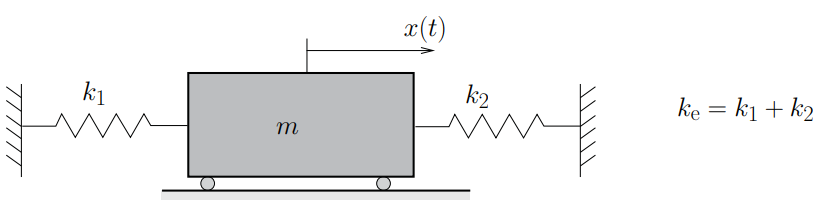
\includegraphics[width=0.5\textwidth]{Sections/Figures/theory spring mass.png}
    \caption{Spring-Mass System}
    \label{fig:Spring-Mass-Damper System}
\end{figure}
If $x$ is the displacement of the mass from its equilibrium position, the equation of motion is given by
\begin{equation}
    m_e\ddot{x} + k_ex = 0 \label{eq:Free Vibration Differential Equation}
\end{equation}
The solution to Equation \ref{eq:Free Vibration Differential Equation} is given by
\begin{equation}
    x(t) = \frac{v_0}{p}\sin(pt) + x_0\cos(pt) \label{eq:Free Vibration Solution}
\end{equation}
where $v_0$ is the initial velocity, $x_0$ is the initial displacement, and $p = \sqrt{\frac{k_e}{m_e}}$ is the natural frequency of the system. The natural frequency is the frequency at which the system will oscillate if it is displaced and released. The period of the system is given by
\begin{equation}
    \tau = \frac{2\pi}{p} \label{eq:Free Vibration Period}
\end{equation}
\subsection{Forced Vibrations}
The experimental setup for forced vibrations is modelled in Figure \ref{fig:Forced Vibrations System Theoretical}. The system consists of a mass $m_e$ attached to a spring with stiffness $k_e$. The force is $F(t) = kY_0\sin(\omega t)$.
\begin{figure}[H]
    \centering
    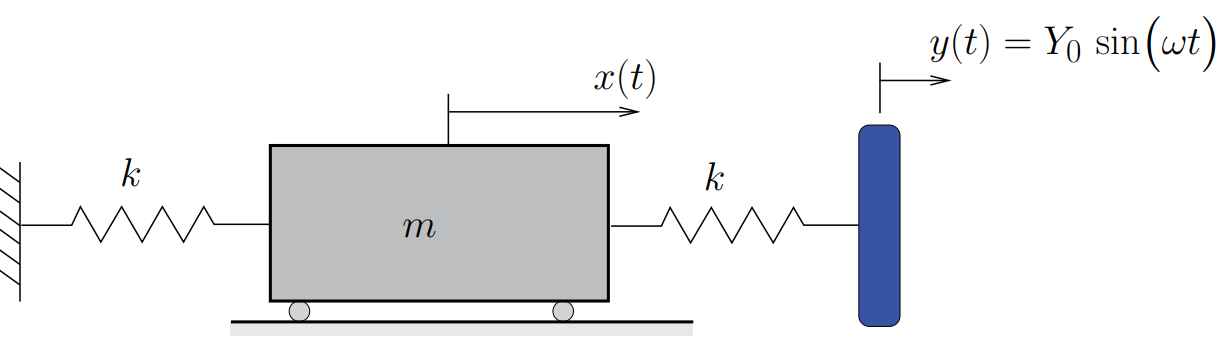
\includegraphics[width=0.5\textwidth]{Sections/Figures/theory forced spring mass.png}
    \caption{Forced Damped Vibrations System}
    \label{fig:Forced Vibrations System Theoretical}
\end{figure}
The equation of motion for the system is given by
\begin{equation}
    m_e\ddot{x} + k_ex = F_0\cos(\omega t) \label{eq:Forced Vibration Differential Equation}
\end{equation}
where $F_0 = kY_0$. The time-dependent solution to Equation \ref{eq:Forced Vibration Differential Equation} is 
\begin{align}
    x(t) &= \frac{Y_0}{2} \left[\frac{1}{1 - \left(\frac{\omega}{p}\right)^2}\right]\sin(\omega t) \label{eq:Forced Vibration Solution} \\
\end{align}
where $p = \sqrt{\frac{k_e}{m_e}}$ is the natural frequency of the system. The DMF is given by
\begin{equation}
    \text{DMF} = \frac{1}{\left|1 - \left(\frac{\omega}{p}\right)^2\right|} \label{eq:DMF}
\end{equation}
Plotting the DMF against $\omega/p$ will give the frequency response of the system, as shown in Figure \ref{fig:DMF}. At $\omega/p< \sqrt{2}$, the DMF $>1$, which means the system amplifies the input force. At $\omega/p > \sqrt{2}$, the DMF $<1$, which means the system attenuates the input force. The system is in resonance at $\omega/p = 1$.
\begin{figure}[h]
    \centering
    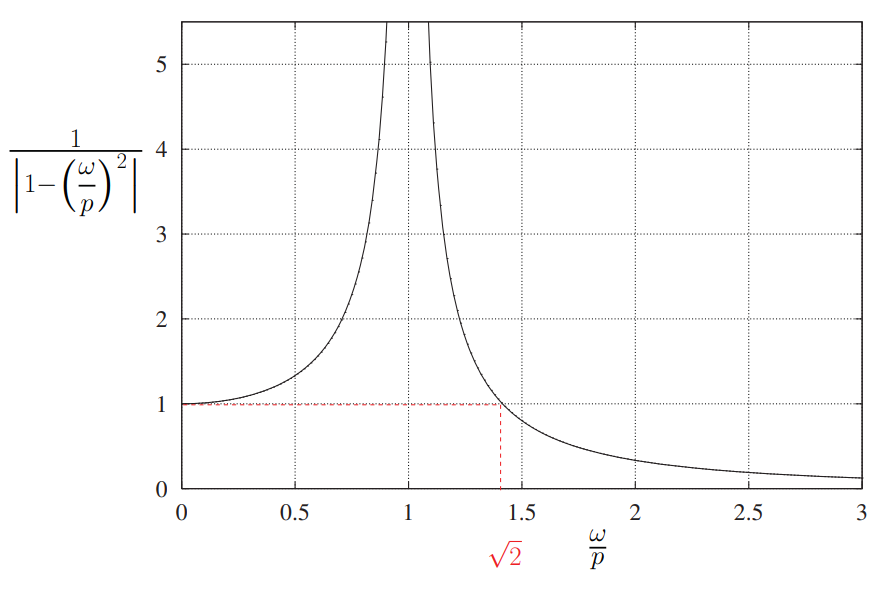
\includegraphics[width=0.5\textwidth]{Sections/Figures/DMF.png}
    \caption{DMF vs. $\omega/p$}
    \label{fig:DMF}
\end{figure}
Defining static deflection as 
\begin{equation}
    \mathbb{X}_0 = \frac{F_0}{k_e} \label{eq:Static Deflection}
\end{equation}
we can see that the $Y_0/2$ term in Eq. \ref{eq:Forced Vibration Solution} is static deflection.

\subsection{Damped Spring Mass System}
\begin{figure}[h]
    \centering
    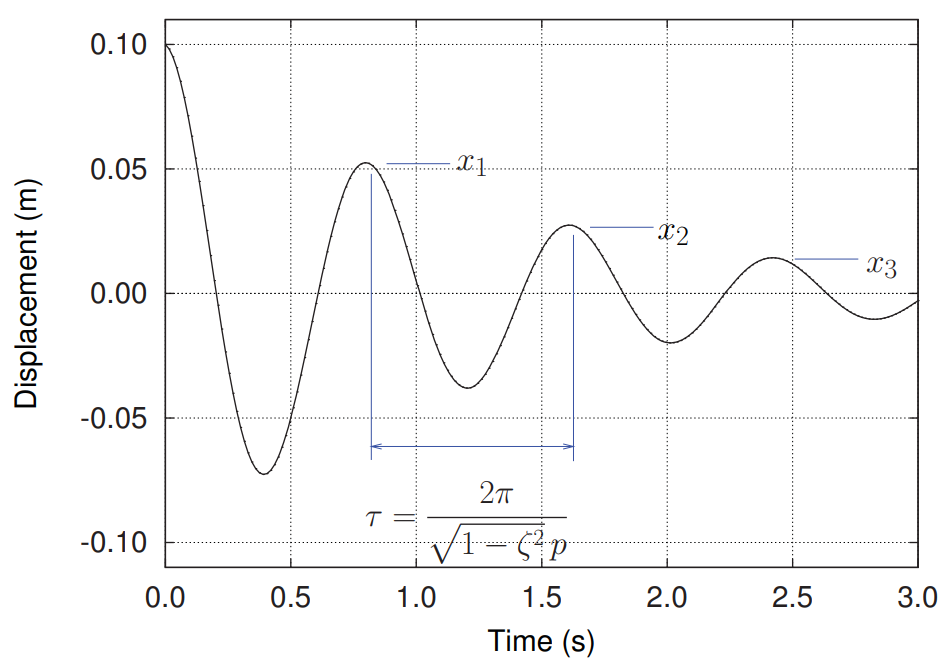
\includegraphics[width=0.5\textwidth]{Sections/Figures/damped response.png}
    \caption{Damped Response of a Spring-Mass System}
    \label{fig:Damped Response}
\end{figure}
An energy dissipation method is added to the system to model the energy loss in the system. The most common approach is to add viscous damping, which is proportional to the velocity of the mass. The equation of motion from Eq. \ref{eq:Free Vibration Differential Equation} is modified to include damping as
\begin{equation}
    m_e\ddot{x} + c_e\dot{x} + k_ex = 0 \label{eq:Damped Vibration Differential Equation}
\end{equation}
where $c_e$ is the damping coefficient. Assuming the mass is given an initial displacement and zero initial velocity, the solution to Eq. \ref{eq:Damped Vibration Differential Equation} is given by
\begin{equation}
    x(t) = A e^{\- \zeta t}\cos\left(\sqrt{1 - \zeta^2}t \right) \label{eq:Damped Vibration Solution}
\end{equation}
where, 
\begin{equation}
    \zeta = \frac{c_e}{2m_e p} = \frac{c_e}{2\sqrt{k_e m_e}} \label{eq:Damping Ratio}
\end{equation}
The solution to Eq. \ref{eq:Damped Vibration Differential Equation} is a decaying sinusoidal function, plotted in Figure \ref{fig:Damped Response}. It can be shown that the peaks can be related by
\begin{align}
    \delta = \ln \left(\frac{x_{n}}{x_{n+1}}\right) = \frac{2\pi}{\sqrt{1 - \zeta^2}} \label{eq:Decay Ratio Delta} 
\end{align}
From which, the damping ratio can be determined as 
\begin{align}
    \zeta = \frac{\delta}{\sqrt{4\pi^2 + \delta^2}} \label{eq:Damping Ratio Calculated With Delta}
\end{align}


\subsection{Equivalent Mass of Measurement System}
\label{sec:Equivalent Mass}
A schematic of the measurement system is shown in Figure \ref{fig:Measurement System}. The equivalent mass of the system is given by
\begin{figure}[H]
    \centering
    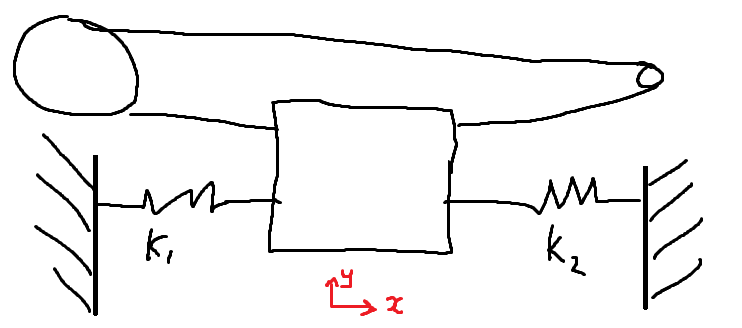
\includegraphics[width=0.5\textwidth]{Sections/Figures/system.png}
    \caption{Cart and Pulley Measurement System}
    \label{fig:Measurement System}
\end{figure}
\begin{figure}[h]
    \centering 
    \begin{minipage}{0.45\textwidth}
        \centering
        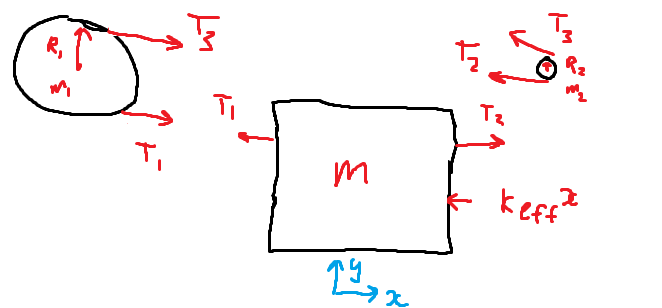
\includegraphics[width=0.9\textwidth]{Sections/Figures/fbd.png}
        \caption{Free Body Diagram of the Cart and Pulleys}
        \label{fig:Cart FBD}
    \end{minipage}\qquad
    \begin{minipage}{0.45\textwidth}
        \centering
        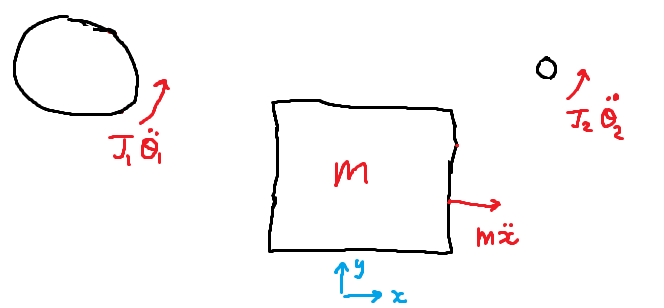
\includegraphics[width=0.9\textwidth]{Sections/Figures/mad.png}
        \caption{Mass Acceleration Diagram of the Cart and Pulleys}
        \label{fig:Cart MAD}
    \end{minipage}  
\end{figure}
Taking the sum of forces in $x$, the moment about pulley 1's and pulley's 2 mass center, 
\begin{align}
    \rightarrow \sum F_x &:= m_{\text{cart}} \ddot{x} \nonumber \\
    &=  T_2 - T_1 - k_{\text{eff}}x \label{eq:Cart Force in x} \\
    \circlearrowleft \sum M_{\text{pulley 1}} &:= J_1 \ddot{\theta}_1 \nonumber \\
    &= R_1 (T_1 - T_3) \label{eq:Pulley 1 Moment} \\
    \circlearrowleft \sum M_{\text{pulley 2}} &:= J_2 \ddot{\theta}_2 \nonumber \\
    &= R_2 (T_3 - T_2) \label{eq:Pulley 2 Moment}
\end{align}
Assuming the cable does not slip,
\begin{align}
    \theta_1 &= \frac{\ddot{x}}{R_1}, \quad \theta_2 = \frac{\ddot{x}}{R_2} \label{eq:Kinematic pure rotation for theta1 and theta2}
\end{align}
Since the disks are uniform disks,
\begin{align}
    J_1 &= \frac{1}{2} m_{1} R_1^2, \quad J_2 = \frac{1}{2} m_{2} R_2^2 \label{eq:Moment of Inertia of Pulleys}
\end{align}
Combining Eq. (\ref{eq:Cart Force in x}), (\ref{eq:Pulley 1 Moment}), (\ref{eq:Pulley 2 Moment}) and using Eq. (\ref{eq:Kinematic pure rotation for theta1 and theta2}) and (\ref{eq:Moment of Inertia of Pulleys}), we get
\begin{align}
    \underbrace{\left(m_{\text{cart}} + \frac{1}{2} m_{1} + \frac{1}{2} m_{2}\right)}_{m_e} \ddot{x} + k_{\text{eff}}x = 0 \label{eq:Equivalent Mass Equation of Motion}
\end{align}
where $m_e$ is the equivalent mass of the system. A full derivation is shown in Appendix \ref{app:Equivalent Mass Derivation}.